% =============================================================================
%  Soutenance CHPS_0805 - Resolution de problemes d'optimisation combinatoire
%  Beamer/Metropolis - format 16:9
% =============================================================================
\documentclass[aspectratio=169, 11pt]{beamer}

\usepackage[utf8]{inputenc}
\usepackage[T1]{fontenc}
\usepackage[french]{babel}
\usepackage{lmodern}
\usepackage{graphicx}
\usepackage{booktabs}
\usepackage{xcolor}
\usepackage{colortbl}
\usepackage{listings}
\usepackage{tikz}
\usepackage{amsmath, amssymb}
\usepackage{microtype}
\usepackage{textcomp}
\usepackage{upquote}

\usetheme{metropolis}
\metroset{
  progressbar=frametitle,
  numbering=fraction,
  block=fill,
  titleformat=smallcaps,
}

% --- Couleurs (alignees avec le rapport et matplotlib) ----------------------
\definecolor{primary}{RGB}{31, 119, 180}
\definecolor{accent}{RGB}{255, 127, 14}
\definecolor{success}{RGB}{44, 160, 44}
\definecolor{warning}{RGB}{214, 39, 40}
\definecolor{codegray}{RGB}{245, 245, 245}

\setbeamercolor{progress bar}{fg=primary}
\setbeamercolor{title separator}{fg=primary}
\setbeamercolor{frametitle}{bg=primary, fg=white}
\setbeamercolor{alerted text}{fg=accent}

% --- Listings ---------------------------------------------------------------
\lstset{
  basicstyle=\ttfamily\scriptsize,
  backgroundcolor=\color{codegray},
  frame=single,
  framesep=3pt,
  rulecolor=\color{black!20},
  numbers=left,
  numberstyle=\tiny\color{black!50},
  numbersep=6pt,
  keywordstyle=\color{primary}\bfseries,
  commentstyle=\color{success}\itshape,
  stringstyle=\color{accent},
  showstringspaces=false,
  breaklines=true,
  tabsize=4,
  upquote=true,
  literate={"}{\textquotedbl}1
           {'}{\textquotesingle}1
           {`}{\textasciigrave}1,
}

% --- Metadonnees ------------------------------------------------------------
\title{Résolution de problèmes d'optimisation combinatoire avec OR-Tools}
\subtitle{Étude comparative Branch \& Bound (C/GLPK) $\leftrightarrow$ OR-Tools (Python)}
\author{Nicolas MARANO}
\institute{\textsc{Université de Reims Champagne-Ardenne} \\ UFR Sciences Exactes et Naturelles --- Master CHPS \\[0.3em] {\small CHPS\_0805 --- Optimisation combinatoire}}
\date{12 mai 2026}

% =============================================================================
\begin{document}
% =============================================================================

% --- Slide 1 : Page de garde -------------------------------------------------
\maketitle

% --- Slide 2 : Plan ----------------------------------------------------------
\begin{frame}{Plan de la présentation}
\tableofcontents[hideallsubsections]
\end{frame}

% =============================================================================
\section{Contexte}
% =============================================================================

% --- Slide 3 : Contexte ------------------------------------------------------
\begin{frame}{Contexte du projet}
\textbf{Cadre} : projet final du cours CHPS\_0805, articulé autour des TP~3 et~5.

\vspace{0.3em}
\textbf{Objectif} : comparer rigoureusement deux familles de méthodes sur deux problèmes \alert{NP-difficiles} classiques.

\vspace{0.6em}
\begin{columns}[T]
\begin{column}{0.5\textwidth}
\begin{block}{Problèmes traités}
\begin{itemize}
  \item \textbf{TSP} --- Voyageur de Commerce
  \item \textbf{UKP} --- Sac à Dos Généralisé
\end{itemize}
\end{block}
\end{column}
\begin{column}{0.5\textwidth}
\begin{block}{Méthodes comparées}
\begin{itemize}
  \item \textbf{B\&B} --- Séparation-Évaluation \\ {\small (C + GLPK, TP3+TP5)}
  \item \textbf{OR-Tools} --- Google \\ {\small (Python : \texttt{pywraplp} + \texttt{pywrapcp})}
\end{itemize}
\end{block}
\end{column}
\end{columns}

\vspace{0.6em}
\textbf{Livrables} : 2 applications unifiées, 22~instances testées, 140+~exécutions chronométrées, 7~figures, audit qualité automatique.
\end{frame}

% --- Slide 4 : Problemes -----------------------------------------------------
\begin{frame}{Les deux problèmes}
\begin{columns}[T]
\begin{column}{0.5\textwidth}
\begin{block}{TSP (minimisation)}
Étant donné $n$ villes et la matrice de distances $d(i,j)$, trouver le \emph{cycle hamiltonien} de longueur minimale~:
\[
  \min \sum_{i=1}^{n} d(\sigma(i), \sigma(i\!+\!1))
\]
où $\sigma$ est une permutation de $\{0,\ldots,n-1\}$ avec $\sigma(n) = \sigma(0)$.
\end{block}
\textbf{Tailles testées} : $n \in [5, 13\,509]$.
\end{column}
\begin{column}{0.5\textwidth}
\begin{block}{UKP (maximisation)}
Étant donnés $n$ objets de volume $v_i$ et utilité $u_i$, capacité $c$~:
\[
  \max \sum_{i=1}^{n} u_i \, x_i \quad \text{s.c.} \quad \sum_{i=1}^{n} v_i \, x_i \leq c, \; x_i \in \mathbb{N}
\]
Variables \alert{entières non bornées} ($x_i \geq 0$).
\end{block}
\textbf{Tailles testées} : $n \in [3, 20\,000]$.
\end{column}
\end{columns}

\vspace{0.4em}
\begin{alertblock}{Difficulté}
NP-difficile dans les deux cas $\Rightarrow$ pas d'algorithme polynomial connu.
\end{alertblock}
\end{frame}

% =============================================================================
\section{Architecture du projet}
% =============================================================================

% --- Slide 5 : Architecture --------------------------------------------------
\begin{frame}[fragile]{Structure du projet}
Deux applications \alert{unifiées et paramétrables}, structure conforme aux modalités~:

\begin{lstlisting}[basicstyle=\ttfamily\tiny]
Simplexe/
|-- README.md
|-- Separation-Evaluation/    # Application C (TP3 + TP5)
|   |-- Makefile, README.md
|   |-- include/   *.h
|   `-- src/       *.c        # main, parser_ukp/tsp, ukp_bb, tsp_bb, ...
|-- OR-Tools/                 # Application Python
|   |-- main.py, README.md, requirements.txt
|   `-- src/       *.py       # parsers, ukp_solver, tsp_solver, visualisation
|-- Resultats/
|   `-- benchmarks_pousses/   # CSV, 7 figures, ANALYSE.md
|-- Romeo/                    # Kit de deploiement HPC URCA (bonus)
`-- scripts/                  # Pipeline automatise
\end{lstlisting}

\begin{itemize}
  \item Compilation C \alert{0 warning} avec 15~flags GCC stricts.
  \item Imports Python \alert{0 warning} sous \texttt{-W~error}.
  \item CLI unifié~: \texttt{./solveur -{}-probleme \{ukp|tsp\} -{}-fichier <chemin>}.
\end{itemize}
\end{frame}

% =============================================================================
\section{Méthodes par séparation-évaluation}
% =============================================================================

% --- Slide 6 : B&B UKP -------------------------------------------------------
\begin{frame}{Branch \& Bound : UKP (TP3)}
\begin{columns}[T]
\begin{column}{0.55\textwidth}
\textbf{Borne initiale} \\
Heuristique \alert{qualité-prix}~: tri par $u_i / v_i$ décroissant, saturation gloutonne.

\vspace{0.5em}
\textbf{Évaluation d'un nœud} \\
Relaxation linéaire par GLPK (\texttt{glp\_simplex}). \\
LP racine captée dans \texttt{stats.lp\_racine}.

\vspace{0.5em}
\textbf{Test d'intégrité} \\
\texttt{modf} sur chaque $x_j$, $\epsilon = 10^{-6}$. \\
Vérification additionnelle de faisabilité.

\vspace{0.5em}
\textbf{Stratégie} \\
DFS itératif sur pile explicite. \\
Séparation~: variable fractionnaire $\to$ branches sur $[0, \lfloor v_{max} \rfloor]$.
\end{column}
\begin{column}{0.45\textwidth}
\begin{block}{Borne LP serrée}
Pour $n \geq 10$ sur les jeux UKP livrés~:
\[
  \text{gap LP--INT} < 0{,}005~\%
\]
$\Rightarrow$ pruning \emph{très peu efficace}, $\Rightarrow$ explosion en temps (millions de nœuds).
\end{block}

\begin{exampleblock}{Validation}
Sur les 9 UKP testables par DP exhaustive~: \\
\textbf{B\&B trouve la valeur optimale} sur les 9 instances.
\end{exampleblock}
\end{column}
\end{columns}
\end{frame}

% --- Slide 7 : B&B TSP -------------------------------------------------------
\begin{frame}{Branch \& Bound : TSP (TP5)}
\begin{columns}[T]
\begin{column}{0.55\textwidth}
\textbf{Borne initiale} \\
Heuristique du \alert{plus proche voisin} depuis le sommet~0 ($O(n^2)$).

\vspace{0.4em}
\textbf{Fonction d'évaluation}~:
\begin{enumerate}\setlength\itemsep{-0.15em}
  \item ACPM (Prim) sur $G \setminus \{0\}$.
  \item + 2 arêtes les plus légères en~0.
\end{enumerate}

\vspace{0.4em}
\textbf{Test} : tous les degrés $= 2$. \\
\textbf{Séparation} : sommet de degré $> 2$ \\ $\to$ trois fils (interdiction d'arête).

\vspace{0.4em}
\textbf{Stratégie} : \alert{meilleur-d'abord} \\ (tas binaire min-heap).

\vspace{0.4em}
\textbf{Bonus 2-opt} : post-traitement.
\end{column}
\begin{column}{0.45\textwidth}
\begin{alertblock}{Limite naturelle}
La borne ACPM décroche dès $n \gtrsim 17$~: \\ l'arborescence explose en $O(N!)$.

Au-delà, OR-Tools s'impose.
\end{alertblock}

\begin{exampleblock}{Convergence observée}
\begin{itemize}\setlength\itemsep{-0.2em}
  \item graphe\_12-15 : ms à secondes
  \item pd\_5/11/15 : ms
  \item pd\_20/22 : 40--52 s
  \item pd\_18, pd\_59+ : timeout
\end{itemize}
\end{exampleblock}
\end{column}
\end{columns}
\end{frame}

% =============================================================================
\section{Méthodes OR-Tools}
% =============================================================================

% --- Slide 8 : OR-Tools UKP --------------------------------------------------
\begin{frame}[fragile]{OR-Tools : UKP via \texttt{pywraplp}}
Solveur MILP \alert{CBC} via la facade \texttt{pywraplp}~:

\begin{lstlisting}[language=Python, basicstyle=\ttfamily\scriptsize]
solver = pywraplp.Solver.CreateSolver("CBC")
variables = [solver.IntVar(0, capacite // volume[j], f"x{j+1}")
             for j in range(n)]
contrainte = solver.Constraint(0, capacite, "capacite")
for j, x in enumerate(variables):
    contrainte.SetCoefficient(x, volume[j])
objectif = solver.Objective()
for j, x in enumerate(variables):
    objectif.SetCoefficient(x, utilite[j])
objectif.SetMaximization()
solver.Solve()
\end{lstlisting}

\vspace{0.3em}
\textbf{Détail clé} : bornes supérieures explicites \texttt{capacite~//~volume[j]} \\
au lieu de \texttt{solver.infinity()} $\Rightarrow$ comportement plus stable sur grandes instances.

\vspace{0.4em}
\textbf{Performances typiques} : prob\_sac\_20000 ($n = 20\,000$) résolu en \alert{1{,}5 s}.
\end{frame}

% --- Slide 9 : OR-Tools TSP --------------------------------------------------
\begin{frame}[fragile]{OR-Tools : TSP via \texttt{pywrapcp.RoutingModel}}
\begin{lstlisting}[language=Python, basicstyle=\ttfamily\scriptsize]
manager = pywrapcp.RoutingIndexManager(n, 1, 0)
routing = pywrapcp.RoutingModel(manager)
def cb(i, j):
    return distances[manager.IndexToNode(i)][manager.IndexToNode(j)]
routing.SetArcCostEvaluatorOfAllVehicles(
    routing.RegisterTransitCallback(cb))

params = pywrapcp.DefaultRoutingSearchParameters()
params.first_solution_strategy = FirstSolutionStrategy.PATH_CHEAPEST_ARC
params.local_search_metaheuristic = LocalSearchMetaheuristic.GUIDED_LOCAL_SEARCH
params.time_limit.seconds = max(1, int(timeout_s))
solution = routing.SolveWithParameters(params)
\end{lstlisting}

\vspace{0.3em}
\textbf{Stratégie} : PATH\_CHEAPEST\_ARC (première solution) + \alert{GUIDED\_LOCAL\_SEARCH} (amélioration).

\vspace{0.4em}
\textbf{Optimisation mémoire} : pour $n > 4\,000$ (canada, usa), bascule automatique sur un calcul de distance \emph{à la volée} (évite une matrice de 5~Go en Python).
\end{frame}

% =============================================================================
\section{Étude expérimentale}
% =============================================================================

% --- Slide 10 : Methodologie -------------------------------------------------
\begin{frame}{Méthodologie du benchmark}
\textbf{Protocole} : multi-répétitions, timeouts adaptatifs, audit automatique.

\vspace{0.3em}
\centering
\small
\begin{tabular}{llccc}
\toprule
\textbf{Catégorie} & \textbf{Instances} & \textbf{Reps} & \textbf{Timeout OR} & \textbf{Timeout BB} \\
\midrule
ukp\_petits  & \texttt{prob\_sac\_1..10}        & 5 & 30~s     & 35~s \\
ukp\_moyens  & \texttt{prob\_sac\_20/25/30}     & 3 & 60~s     & 65~s \\
ukp\_grands  & \texttt{prob\_sac\_2000/20000}   & 2 & 60~s     & 30~s \\
tsp\_petits  & graphe\_12..15, pd\_5/11/15      & 5 & 5~s      & 10~s \\
tsp\_moyens  & pd\_18/20/22                     & 3 & 15~s     & 90~s \\
tsp\_grands  & pd\_59, canada\_4663, usa\_13509 & 2 & 60--180~s & 15--30~s \\
\bottomrule
\end{tabular}

\vspace{0.6em}
\raggedright
\textbf{Audit qualité automatique} :
\begin{itemize}
  \item Croisement BB vs OR-Tools sur chaque instance.
  \item DP exhaustive (oracle) pour les UKP de taille modérée ($n \times c < 10^7$).
  \item Rapport \texttt{OK / WARNING / ERROR} en fin de chaque benchmark.
\end{itemize}
\end{frame}

% --- Slide 11 : Resultats UKP ------------------------------------------------
\begin{frame}{Résultats UKP : crossover et anomalies}
\centering
\scriptsize
\begin{tabular}{lrlll}
\toprule
\textbf{Instance} & $\boldsymbol{n}$ & \textbf{OR-Tools} & \textbf{B\&B (C)} & \textbf{Verdict} \\
\midrule
prob\_sac\_1     & 3     & 13 / 2{,}3 ms      & \textbf{13 / 100 µs}        & = ; BB plus rapide \\
prob\_sac\_5     & 10    & \textbf{199 / 2 ms}     & 199 / 4{,}2 ms          & = ; OR plus rapide \\
prob\_sac\_10    & 10    & \textbf{285\,932 / 13 ms} & 285\,932 / 315 ms      & = ; OR $\times$ 24 \\
\rowcolor{warning!10}
prob\_sac\_20    & 20    & 125\,942 / 44 ms        & \textbf{125\,950 / 8{,}8 s} & \textcolor{warning}{\textbf{BB meilleur}} \\
\rowcolor{warning!10}
prob\_sac\_25    & 25    & 285\,934 / 6{,}7 ms     & \textbf{285\,935 / 178 ms}  & \textcolor{warning}{\textbf{BB meilleur}} \\
prob\_sac\_30    & 30    & \textbf{95\,960 / 9 ms} & 95\,960 / 5{,}9 s            & = ; OR $\times$ 650 \\
prob\_sac\_2000  & 2\,000  & \textbf{1\,029\,627 / 344 ms} & timeout            & OR seul \\
prob\_sac\_20000 & 20\,000 & \textbf{3\,793\,644 / 1{,}5 s} & skip              & OR seul \\
\bottomrule
\end{tabular}

\vspace{0.6em}
\raggedright
\begin{itemize}
  \item Crossover BB/OR autour de $n \approx 4$--$5$.
  \item OR-Tools \alert{$\times$ 650} plus rapide à $n=30$.
  \item \alert{Anomalie CBC} : prob\_sac\_20 et prob\_sac\_25 (à détailler slide suivante).
\end{itemize}
\end{frame}

% --- Slide 12 : Panneau principal --------------------------------------------
\begin{frame}{Vue d'ensemble : panneau principal}
\centering
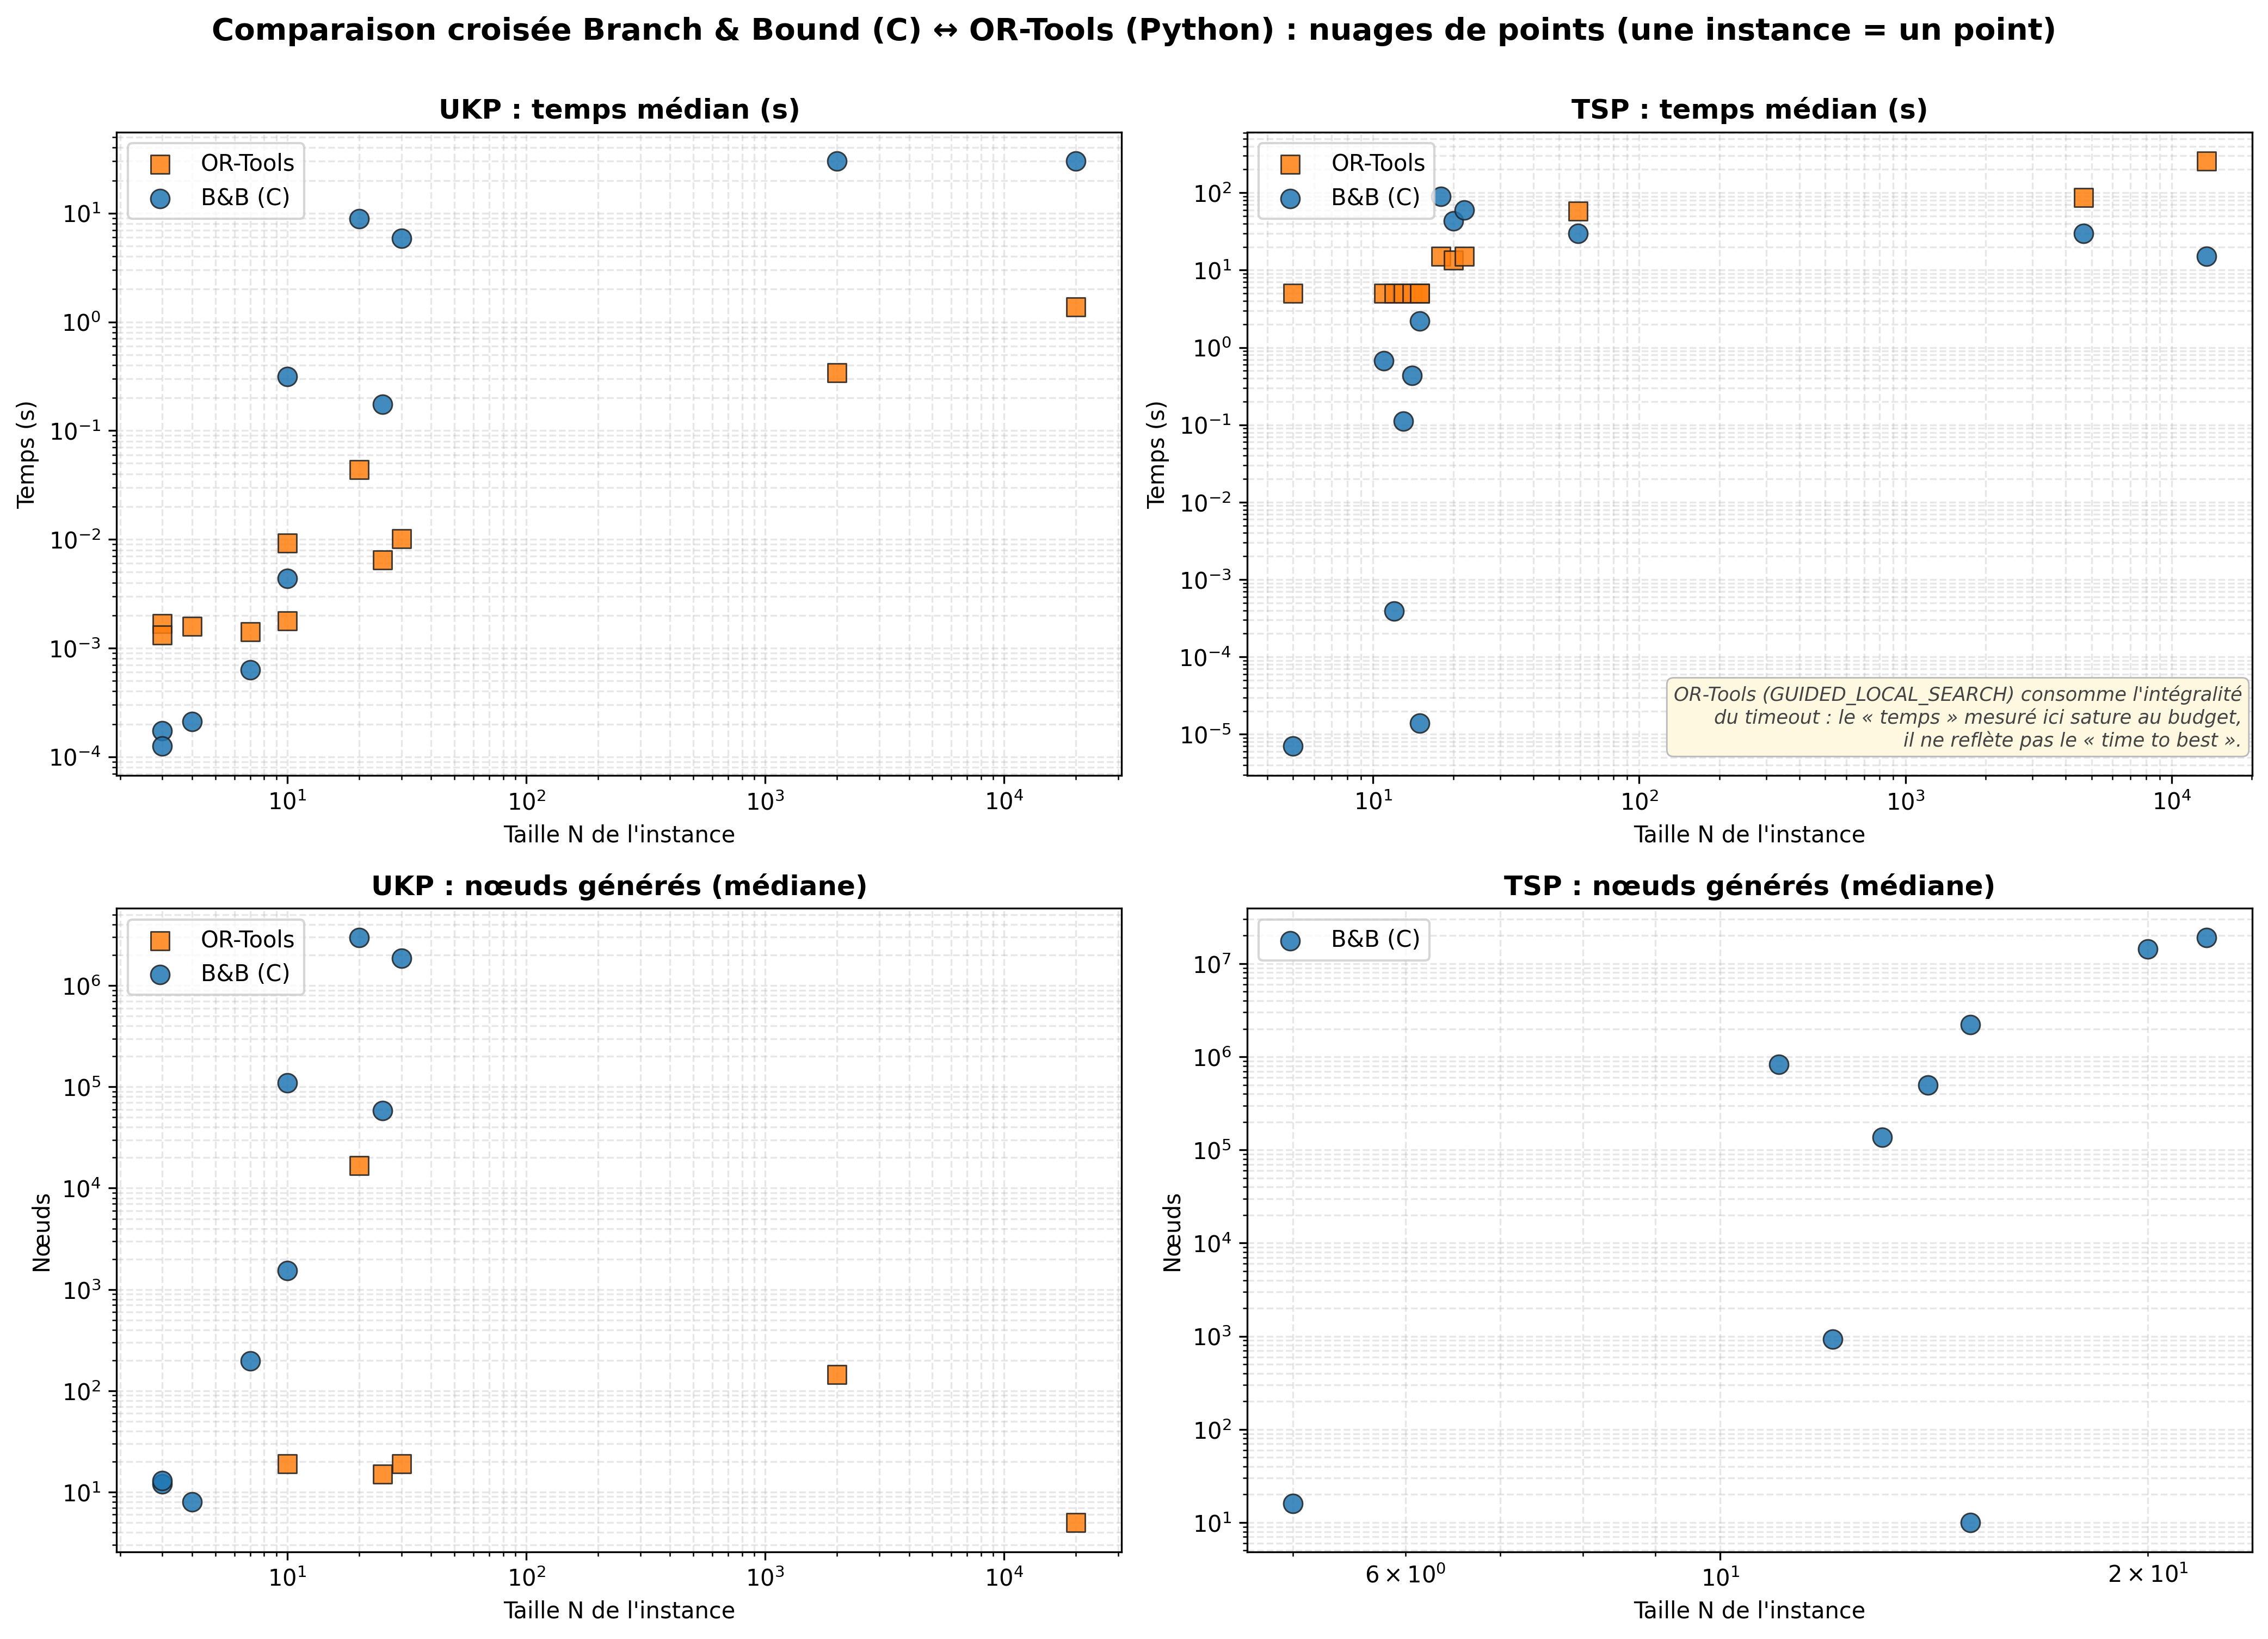
\includegraphics[height=0.78\textheight]{../Resultats/benchmarks_pousses/panneau_principal.png}

\vspace{-0.3em}
{\scriptsize Quatre axes log-log : temps + nœuds $\times$ UKP + TSP. Non-monotonie B\&B révèle la sensibilité au gap LP.}
\end{frame}

% --- Slide 13 : Resultats TSP ------------------------------------------------
\begin{frame}{Résultats TSP}
\centering
\scriptsize
\begin{tabular}{lrlll}
\toprule
\textbf{Instance} & $\boldsymbol{n}$ & \textbf{OR-Tools} & \textbf{B\&B (C)} & \textbf{Verdict} \\
\midrule
graphe\_12    & 12     & 23 / 5 s              & \textbf{23 / 415 µs}     & BB $\times 12\,000$ \\
pd\_5         & 5      & 20 / 5 s              & \textbf{20 / 7 µs}       & BB instantané \\
pd\_15        & 15     & 284 / 5 s             & \textbf{284 / 14 µs}     & BB instantané \\
pd\_18        & 18     & \textbf{268 / 15 s}   & timeout $> 90$ s         & OR seul \\
pd\_20        & 20     & 673 / 15 s            & \textbf{673 / 40 s}      & = ; BB converge \\
pd\_22        & 22     & 788 / 15 s            & \textbf{788 / 52 s}      & = ; BB converge \\
pd\_59        & 59     & \textbf{1\,005 / 60 s} & timeout                  & OR seul \\
canada\_4663  & 4\,663 & \textbf{1\,584\,130 / 90 s} & timeout              & OR seul \\
usa\_13509    & 13\,509 & \textbf{24\,955\,244 / 245 s} & timeout           & OR seul \\
\bottomrule
\end{tabular}

\vspace{0.5em}
\raggedright
\textbf{Limite du B\&B} : optimal jusqu'à $N \approx 17$, encore convergent sur \texttt{pd\_20/22}. \\
\textbf{Force d'OR-Tools} : seul à fournir une solution sur \alert{usa\_13509} (13\,509 villes en 4 min).
\end{frame}

% --- Slide 14 : Visualisation tour -------------------------------------------
\begin{frame}{Visualisation : tour TSP \texttt{pd\_22}}
\centering
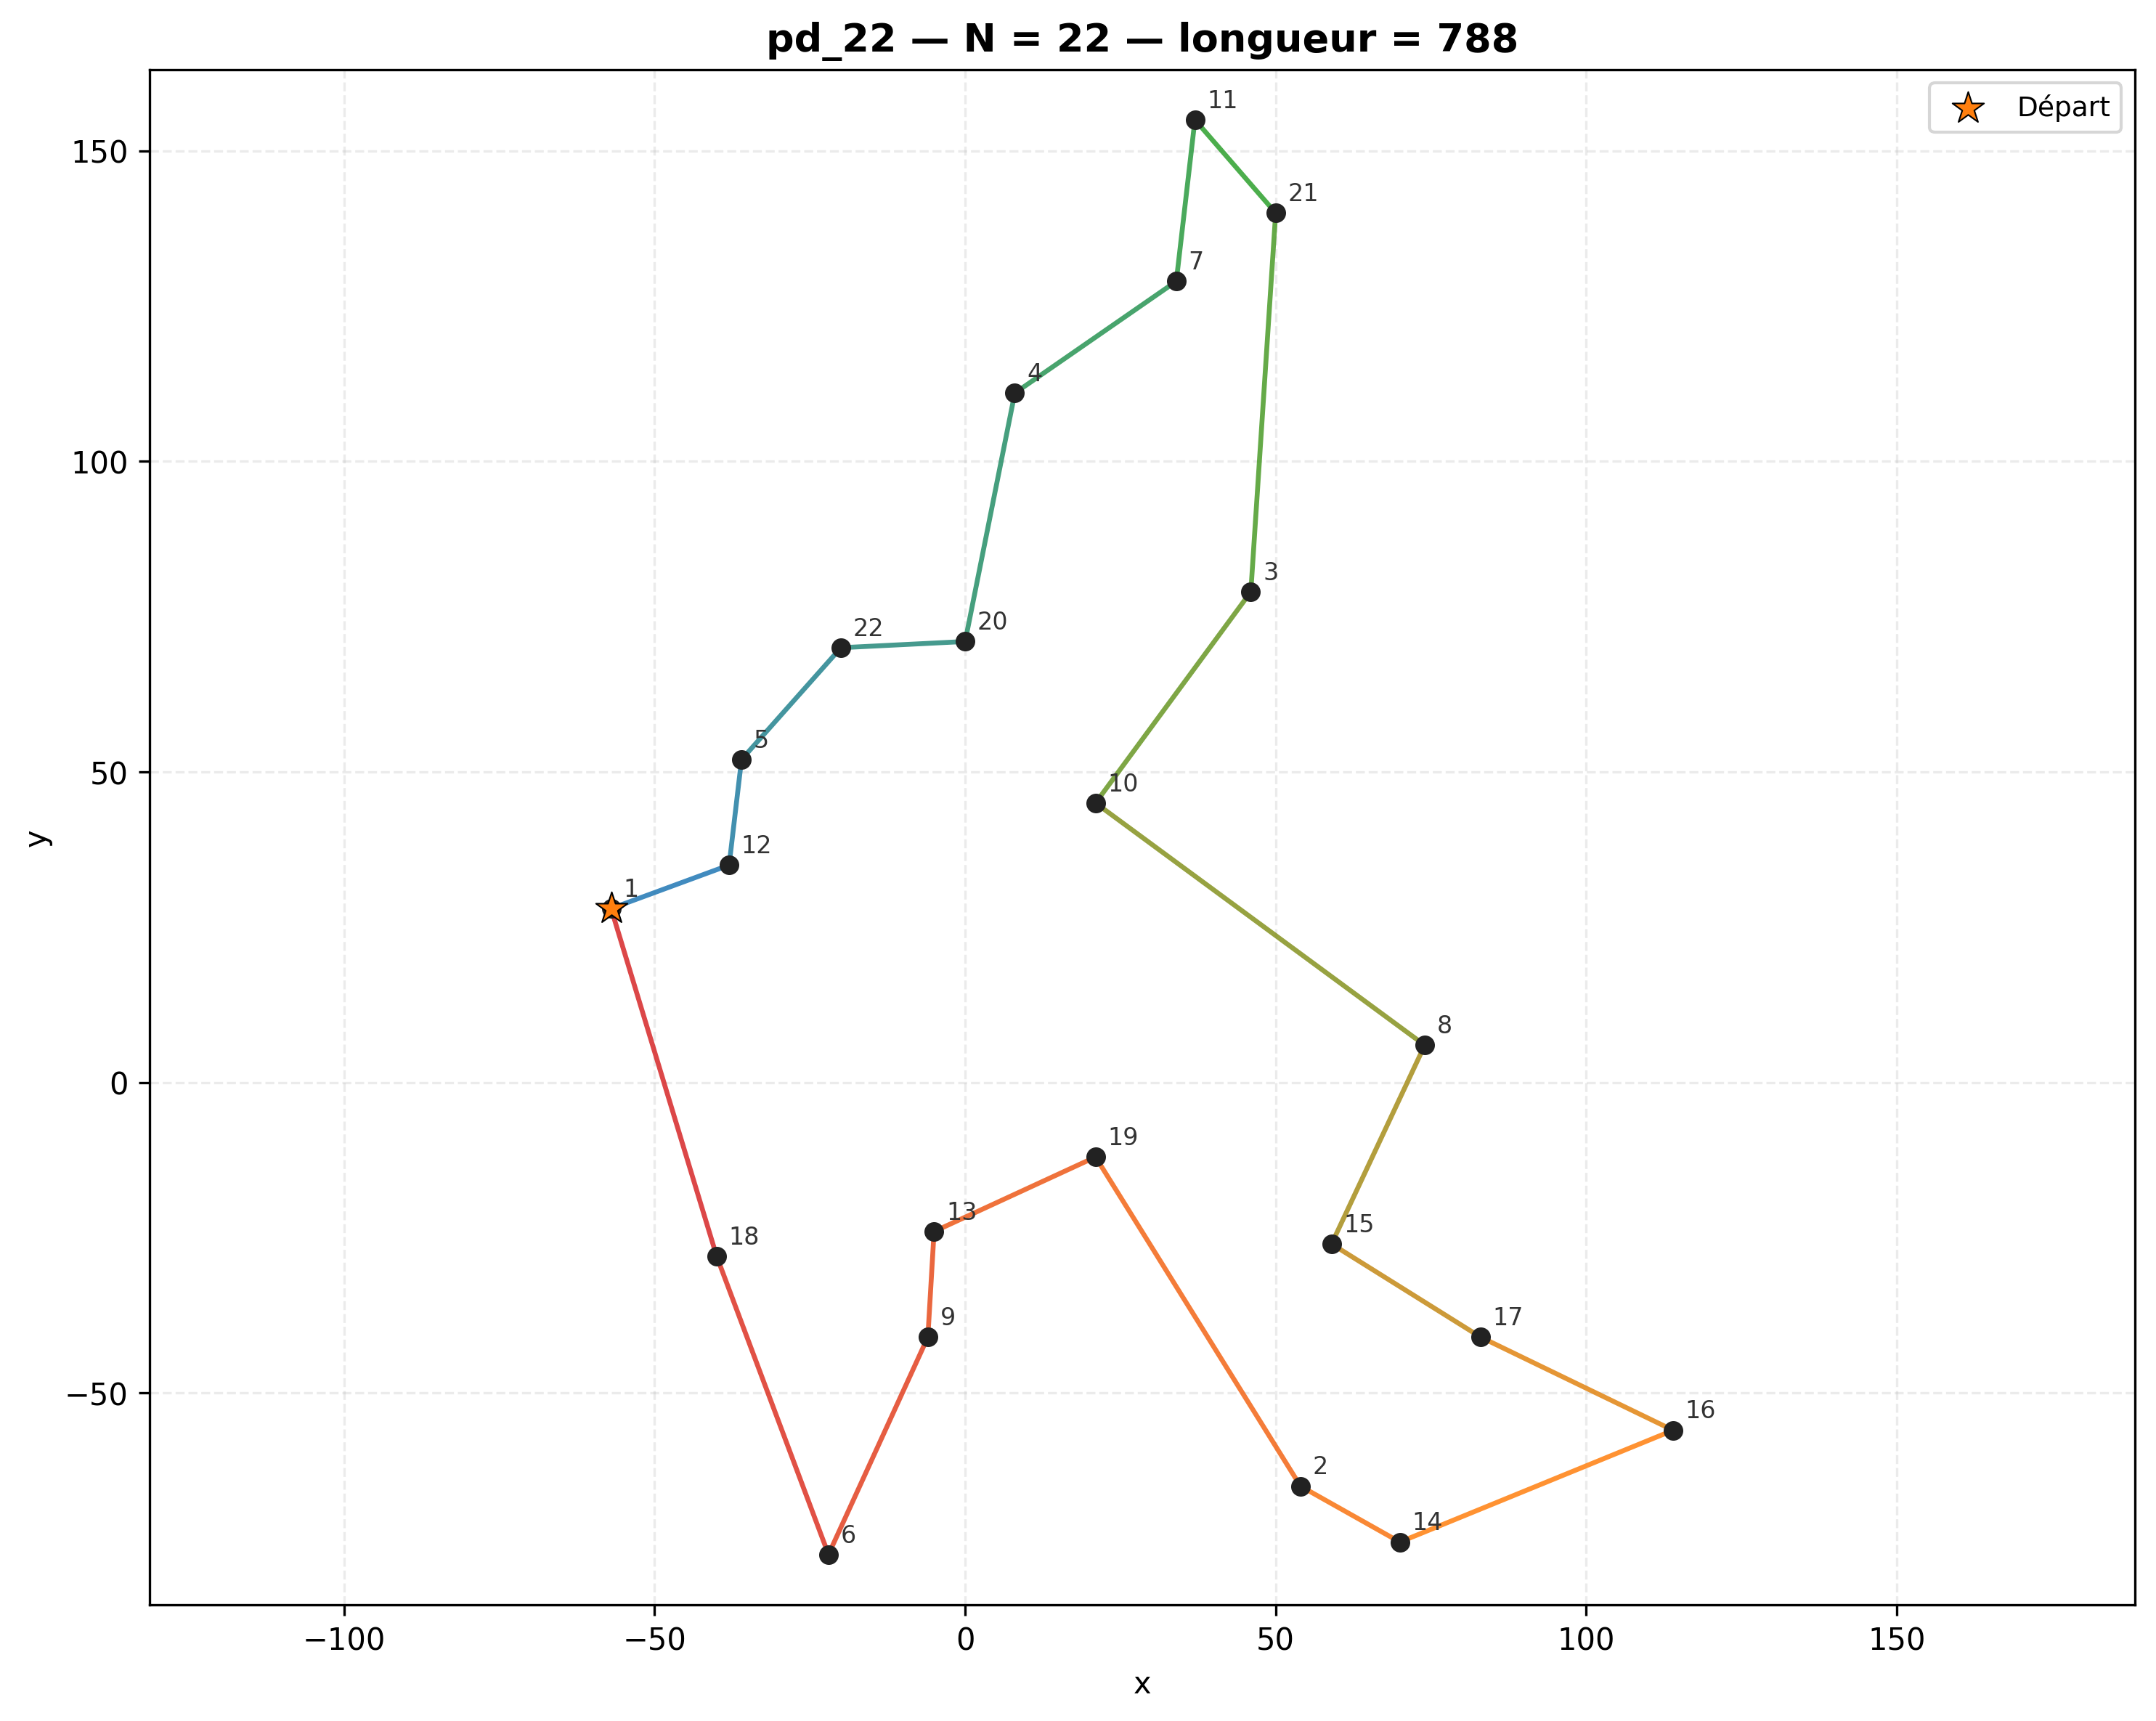
\includegraphics[height=0.8\textheight]{../Resultats/visualisations/tsp_pd_22_tour.png}
\end{frame}

% --- Slide 15 : Anomalies CBC ------------------------------------------------
\begin{frame}{Anomalies CBC détectées et certifiées}
L'audit qualité a révélé deux instances UKP où \alert{CBC renvoie une solution sous-optimale} avec statut \texttt{OPTIMAL} :

\vspace{0.4em}
\centering
\small
\begin{tabular}{lrrrrr}
\toprule
\textbf{Instance} & \textbf{DP (oracle)} & \textbf{B\&B (C)} & \textbf{CBC} & \textbf{Écart} & \textbf{Gap LP--INT} \\
\midrule
\texttt{prob\_sac\_20} & \textbf{125\,950} & \textbf{125\,950}~$\checkmark$ & 125\,942 & $-8$ & $0{,}0023~\%$ \\
\texttt{prob\_sac\_25} & \textbf{285\,935} & \textbf{285\,935}~$\checkmark$ & 285\,934 & $-1$ & $0{,}0004~\%$ \\
\bottomrule
\end{tabular}

\vspace{0.5em}
\raggedright
\begin{itemize}
  \item \textbf{Vérification} : programmation dynamique exhaustive comme oracle indépendant.
  \item \textbf{Cause} : utilités quasi-uniformes ($u_i \approx v_i - 5$), gap LP/INT $< 0{,}005~\%$ \\
        $\Rightarrow$ \texttt{cutoff} numérique CBC trop large.
  \item \textbf{SCIP, BOP} : également sous-optimaux mais sur des valeurs différentes.
\end{itemize}

\vspace{0.4em}
\begin{alertblock}{Enseignement}
\textbf{Aucune méthode n'est universelle.} Le croisement BB $\leftrightarrow$ OR-Tools est crucial pour fiabiliser les résultats.
\end{alertblock}
\end{frame}

% --- Slide 16 : Performance profile ------------------------------------------
\begin{frame}{Profil de performance Dolan--Moré}
\centering
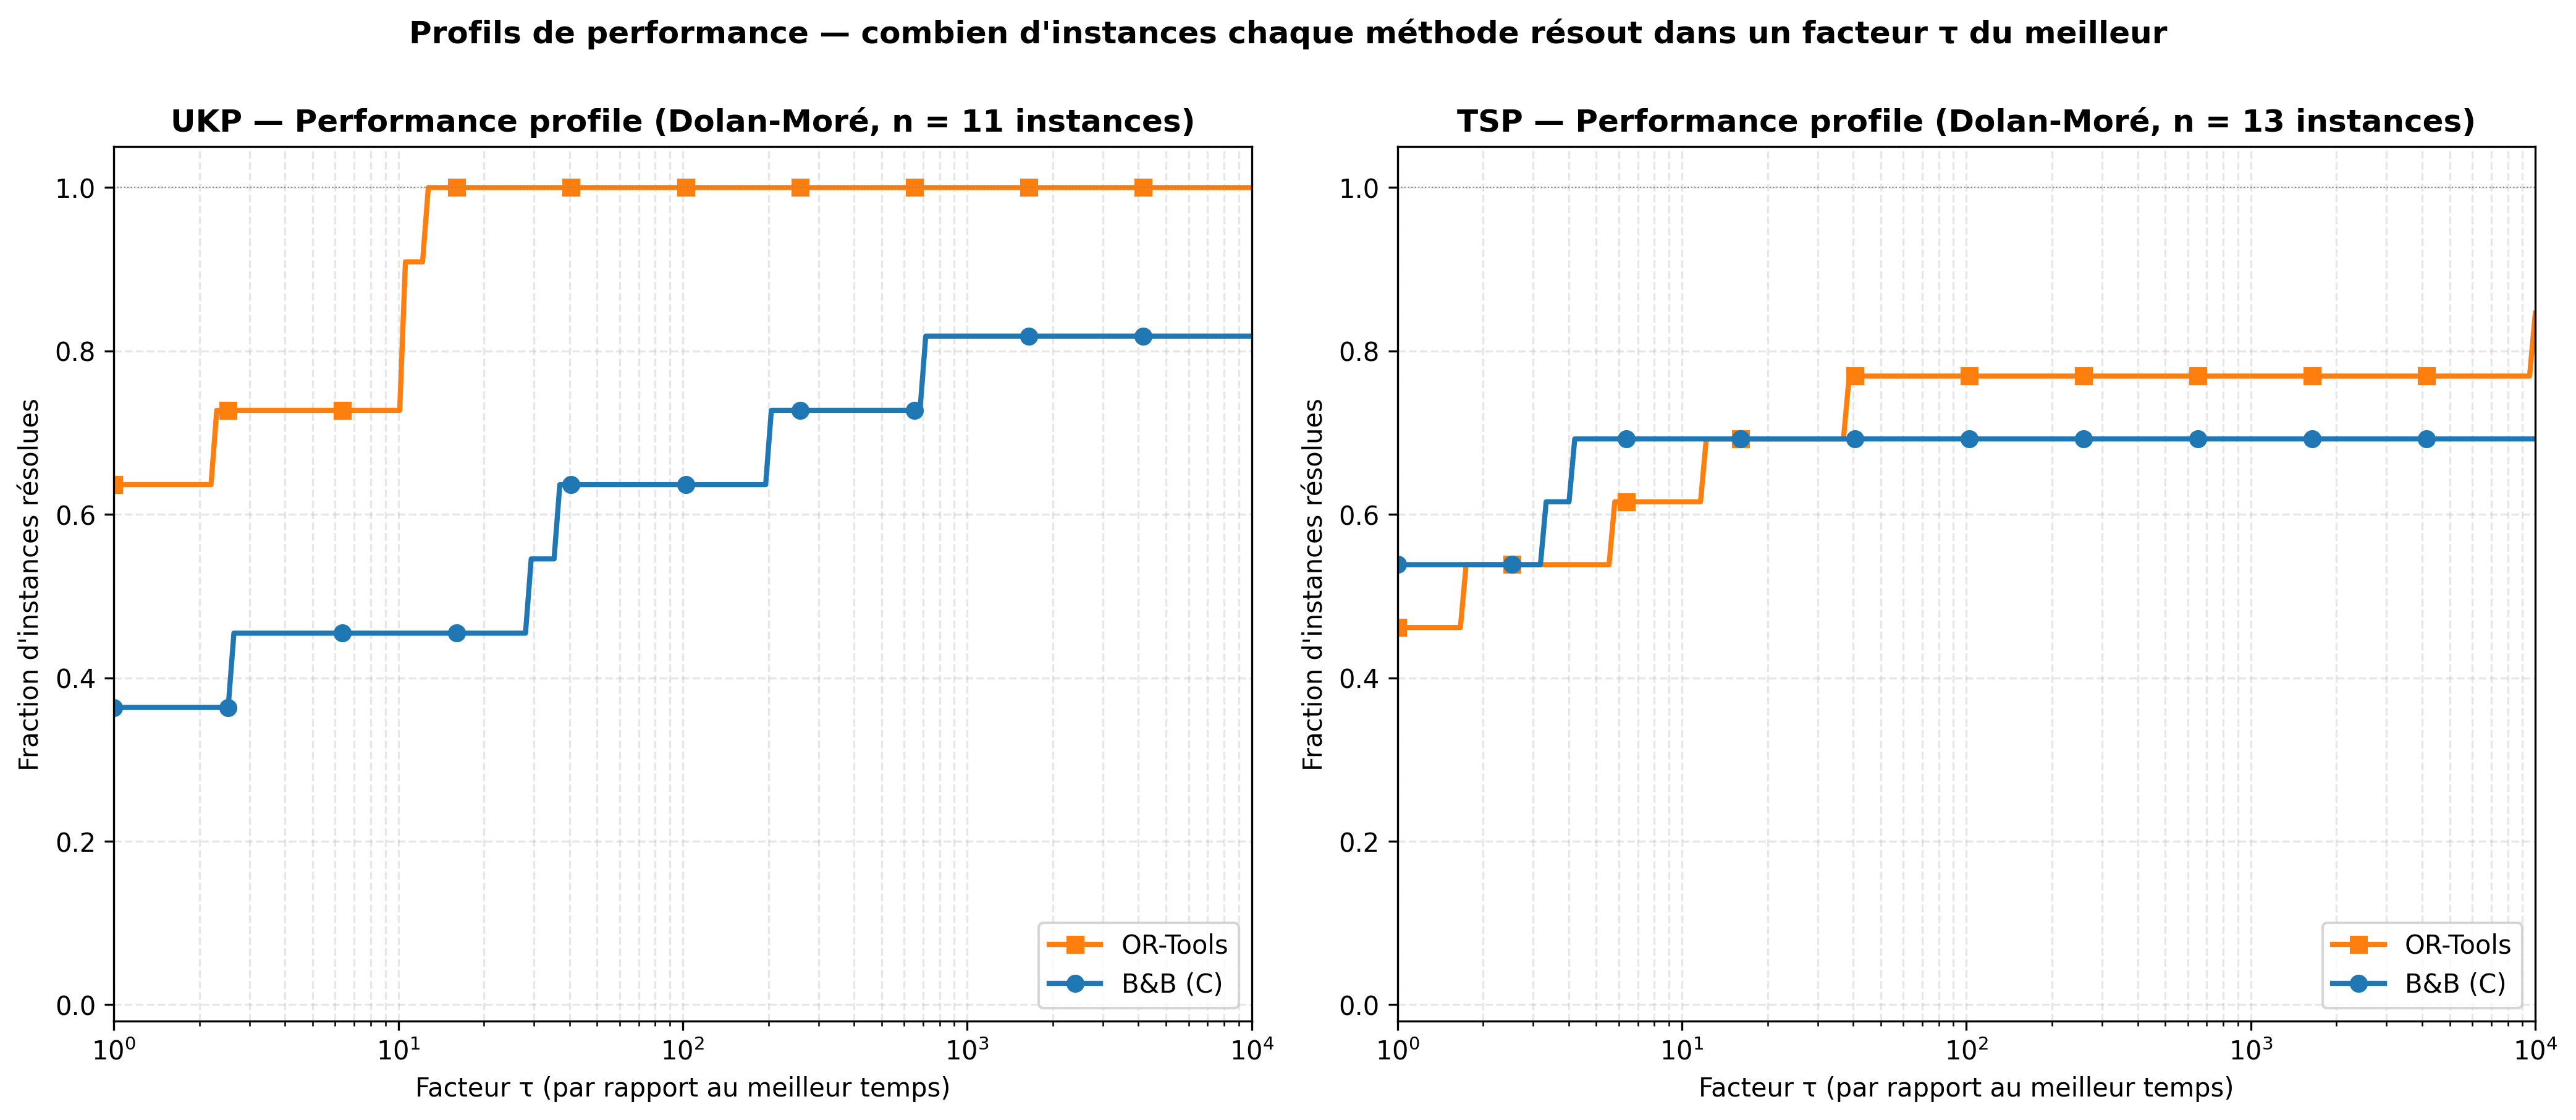
\includegraphics[width=\textwidth]{../Resultats/benchmarks_pousses/performance_profile.png}

\vspace{-0.3em}
{\scriptsize Fraction d'instances résolues dans un facteur $\tau$ du meilleur temps. \\
UKP : OR-Tools domine. TSP : équilibre BB/OR au-delà de $\tau \approx 10$.}
\end{frame}

% =============================================================================
\section{Discussion et conclusion}
% =============================================================================

% --- Slide 17 : Difficultes --------------------------------------------------
\begin{frame}{Difficultés rencontrées}
\begin{itemize}
  \item \textbf{Mémoire pour usa\_13509} : matrice de distances $\approx$~5~Go en Python. \\
        $\Rightarrow$ bascule automatique sur calcul à la volée pour $n > 4\,000$.

  \item \textbf{Anomalies CBC silencieuses} : statut \texttt{OPTIMAL} renvoyé sur des solutions non-optimales. \\
        $\Rightarrow$ détection par audit DP exhaustive automatisé.

  \item \textbf{Timeouts inadaptés} : initialement 15~s sur \texttt{tsp\_moyens} faussait pd\_20/pd\_22. \\
        $\Rightarrow$ correction à 90~s, révélant que ces instances convergent réellement.

  \item \textbf{Trade-off compilateur} : rewrite \texttt{i\,\textless\,n\,-\,1} $\to$ \texttt{i+1\,\textless\,n} pour silencer \texttt{-Wstrict-overflow=5} a coûté $\sim 10~\%$ de performance sur les boucles longues. \\
        $\Rightarrow$ compromis assumé en faveur d'un code certifié \alert{0~warning}.
\end{itemize}
\end{frame}

% --- Slide 18 : Ameliorations ------------------------------------------------
\begin{frame}{Améliorations possibles}
\begin{block}{Algorithmes plus puissants}
\begin{itemize}
  \item \textbf{Borne Held--Karp} pour le TSP : relaxation lagrangienne sur l'ACPM, plus serrée que ACPM seul $\Rightarrow$ étendrait la convergence du B\&B au-delà de $n = 22$.
  \item \textbf{Lin--Kernighan} en métaheuristique côté C : alternative à OR-Tools sur les très grandes instances.
\end{itemize}
\end{block}

\begin{block}{Performance et instrumentation}
\begin{itemize}
  \item \textbf{Parallélisation OpenMP} sur les branches du B\&B UKP ($n \sim 30$).
  \item \textbf{« Time to best »} pour OR-Tools TSP via \texttt{SolutionCollector} : éviter l'artéfact de timeout.
  \item \textbf{Mesure mémoire propre} via \texttt{/usr/bin/time -v} ou \texttt{psutil}.
\end{itemize}
\end{block}
\end{frame}

% --- Slide 19 : Conclusion ---------------------------------------------------
\begin{frame}{Conclusion}
\textbf{Bilan technique} :
\begin{itemize}
  \item \alert{Aucune méthode n'est universellement supérieure}.
  \item B\&B \emph{maison} : déterministe, exact, rapide sur les très petites instances.
  \item OR-Tools : performant sur les instances moyennes/grandes, mais \emph{faillible} numériquement.
\end{itemize}

\textbf{Bonnes pratiques mises en œuvre} :
\begin{itemize}
  \item Audit qualité \alert{automatique} (croisement + DP oracle) à chaque benchmark.
  \item Code \alert{0 warning} sous 15~flags GCC stricts.
  \item Reproductibilité totale : multi-rep, CSV bruts, scripts de pipeline.
  \item Visualisations \emph{publication-ready} : 7 figures pour le rapport.
  \item Préparation \emph{HPC} : kit Romeo (job SLURM, déploiement \texttt{rsync}).
\end{itemize}

\vspace{0.5em}
\centering
\textbf{Toutes les instances obligatoires (Parties 1, 2, 3) ont été traitées.}
\end{frame}

% --- Slide 20 : Demo ---------------------------------------------------------
\begin{frame}[fragile]{Démonstration et questions}
\begin{block}{Commandes pour la démo live}
\begin{lstlisting}[basicstyle=\ttfamily\tiny, language=bash]
# Compilation C
cd Separation-Evaluation && make
./bin/solveur --probleme ukp --fichier "../Fichiers tests*/prob_sac_1.txt" --verbose

# OR-Tools + visualisation
python OR-Tools/main.py --probleme tsp --fichier "../Fichiers tests*/pd_22.tsp" --visu

# Pipeline complet (~2h sur Romeo, ~1h en local)
bash scripts/run_benchmark_pousse.sh --inclure-grands

# Audit qualite (DP exhaustive comme oracle)
bash scripts/_verif_dp_complete.sh
\end{lstlisting}
\end{block}

\vfill
\centering
{\huge \textbf{Merci de votre attention.}} \\[0.6em]
{\Large Questions~?}
\vfill
\end{frame}

\end{document}
